\chapter{Functional Renormalization and Quantum Gravity}\label{chap:EHT}
%TODO: GAUGE FIXING! Faddeev-Popov
%TODO: Have a look at the derivation of the equation.. still some terms missing
\section{Asymptotic Safety}

\section{Einstein-Hilbert Truncation}
We want to solve the Flow equation (\ref{eqn:QGflow}) approximately. All terms that are invariant under the imposed symmetry, i.\,e. invariant under diffeomorphism transformations need to be taken into account. \\

Easiest truncation takes only the scalar curvature $\mathcal{R}$ and the cosmological constant $\Lambda$ into account (No higher order terms \dots) and was performed by Martin Reuter in 1993 \cite{ReuterSaueressig2002}. \\


This truncation reads
\begin{align}
	\Gammak = 2\kappa^2Z_k \int_x \sqrt{g} \ [-\mathcal{R} + 2\Lambda_k] + \mathcal{S}_{\text{gf}} + \mathcal{S}_{\text{gh}}
\label{eqn:QGflow}
\end{align}
with 
\begin{align}
	\kappa^2 = \frac{1}{32\pi G}, \qquad\qquad G_k = GZ^{-1}_k
\end{align}



anomalous dimension: 
\begin{align*}
	\eta_g = -\frac{\partial_t Z_k}{Z_k} = -\partial_t \ln Z_k
\end{align*}

dimensionless renormalized cosmological constant:
\begin{align*}
	\lambda_k = \Lambdak k^{-2}
\end{align*}

dimensionless renormalized cosmological constant:
\begin{align*}
	g_k = G_k k^{d-2} = \frac{Gk^{d-2}}{Z_k}
\end{align*}

corresponding beta function:
\begin{align}
	\beta_g = \partial_t g_k = \left(d-2 + \eta_g\right)g_k
\end{align}

maximally symmetric space:
\begin{align}
	\bar{\mathcal{R}}_{\mu\nu} = \frac{1}{d} \ \bar{g}_{\mu\nu} \bar{\mathcal{R}}
\end{align}
\begin{align}
	\bar{\mathcal{R}}_{\mu\nu\rho\sigma} = \frac{1}{d(d-1)} \ (\bar{g}_{\mu\rho}\bar{g}_{\nu\sigma} - \bar{g}_{\mu\sigma}\bar{g}_{\nu\rho}) \bar{\mathcal{R}}
\end{align}

suitable tensor basis:

%TODO: Adapt this to the definition given in the Appendix 
As a first approximation, we only take the contribution from the spin-two graviton mode $h_{\mu\nu}^{\text{TT}}$ into account. This is motivated by the fact, that this mode carries the the most degrees of freedom.\\ %TODO: Extend this explanation (exercise sheet...)
In this setting, we want to solve the Wetterich equation (\ref{eqn:Wetterich}) by computing the left hand side and the right hand side separately and extract the $\beta$-functions for the Newton coupling $g_k$ and the cosmological constant $\lambda_k$ by a comparison of all terms of order $\sim\sqrt{g}$ and $\sim \sqrt{g} \ \mathcal{R}$. Here, only the most important steps of the calculation are presented. For the complete calculation have a look at Appendix A. \\%TODO:Referencing the Appendix. 
In our spin-two graviton mode approximation, we don't have to deal with the gauge-fixing and ghost parts ocuring in the effective action. The simplified version of equation (\ref{eqn:QGflow}) reads
\begin{align}
	\Gamma_{k, h^{\text{TT}}} = 2\kappa^2Z_k \int_x \sqrt{g} \ [-\mathcal{R} + 2\Lambda_k].
\end{align}
We start by computing the transverse-traceless graviton two-point function
\begin{align}
\Gamma_{h^{\text{TT}}h^{\text{TT}}}^{(2)} = \frac{Z_k}{32\pi}\left(\bar{\Delta} - 2\Lambda_k+\frac{2}{3}\bar{\mathcal{R}}\right).
\end{align}
Using a regulator of the form
\begin{align}
R_k  = \eval{\Gamma_{h^{\text{TT}}h^{\text{TT}}}^{(2)}}_{\Lambda_k=\bar{\mathcal{R}}=0} \cdot r_k\left(\frac{\bar{\Delta}}{k^2}\right) = \frac{Z_k}{32\pi}\bar{\Delta}\left(\frac{k^2}{\bar{\Delta}}-1\right)\Theta\left(1-\frac{\bar{\Delta}}{k^2}\right), \nonumber
\end{align}
with a Litim-type cutoff
\begin{align}
r_k(y) = \left(\frac{1}{y}-1\right)\Theta(1-y), \label{eqn:Litim}
\end{align}
as discussed in chapter (\ref{chap:QFT}), we are directly able to compute the l.\,h.\,s. of the Wetterich equation, i.\,e. the scale derivative of the effective average action:
\begin{align}
	\partial_{t}\Gamma_{k,h^{\text{TT}}} = 2\kappa^2 Z_k\int_x \sqrt{g} \left\{\eta_g\mathcal{R}+2\left(k^2(\partial_t\lambda_k) + \Lambda_k(2 - \eta_g)\right)\right\}
\end{align}
One can extract the $\beta$-function for the Newton coupling without performing the analysis of the Wetterich equation, i.\,e. 
\begin{align}
\beta_g = \partial_t g_k = \partial_t\left(\frac{G\cdot k^2}{Z_k}\right) = g_k\left(2+\eta_g\right).
\end{align}

The computation of the r.\,h.\,s. of the flow equation is more complicated because it involves the computation of a trace of a function depending on the Laplacian on a curved background. We can use heat-kernel techniques to solve such equations. Heat-kernel computations are based on a curvature expansion in powers of the curvature scaler $\mathcal{R}$. For more details, have a look at the appendix (\ref{sec:heat-kernel}). As a first step, we simplify the trace expression as much as possible.

\begin{align}
\operatorname{Tr}\left[\frac{1}{\Gammak^{(2)} + R_k}\partial_t R_k\right] & = \operatorname{Tr}\left[\frac{\partial_t\left(\frac{Z_k}{32\pi}\bar{\Delta}\right)r_k}{\left(\frac{Z_k}{32\pi}\right)\left(\bar{\Delta} - 2\Lambda_k + \frac{2}{3}\bar{\mathcal{R}}\right) + \left(\frac{Z_k}{32\pi}\bar{\Delta}\right) r_k}\right]	\nonumber \\
\phantom{.} \\
&= \operatorname{Tr}\left[\frac{\bar{\Delta}\left(\partial_t r_k - \eta_g r_k\right)}{\bar{\Delta}(1+r_k)-2\Lambda_k+\frac{2}{3}\bar{\mathcal{R}}}\right] \nonumber
\end{align}

We expand this expression around vanishing curvature and get
\begin{align}
\resizebox{.9 \textwidth}{!}{$
\operatorname{Tr}\left[\frac{1}{\Gammak^{(2)} + R_k}\partial_t R_k\right] = \operatorname{Tr}\left[\frac{\bar{\Delta}\left(\partial_t r_k - \eta_g r_k\right)}{\bar{\Delta}(1+r_k)-2\Lambda_k}\right] - \frac{2}{3}\bar{\mathcal{R}}\operatorname{Tr}\left[\frac{\bar{\Delta}\left(\partial_t r_k - \eta_g r_k\right)}{\left(\bar{\Delta}(1+r_k)-2\Lambda_k\right)^2}\right] + \mathcal{O}(\mathcal{R}^2)$
}
\end{align}
Now we are able to evaluate these two terms separately using heat-kernel techniques. One finds for the first term
\begin{align}
\operatorname{Tr}\left[\frac{\bar{\Delta}\left(\partial_t r_k - \eta_g r_k\right)}{\bar{\Delta}(1+r_k)-2\Lambda_k}\right] = \frac{1}{(4\pi)^2}\int_x \sqrt{g} \left[5\Phi_2^1(-2\Lambda_k) - \frac{5}{6}\bar{\mathcal{R}}\Phi^1_1(-2\Lambda_k)\right],
\end{align}
with the threshold functions 
\begin{align}
	\Phi_n^p(\omega) = \frac{1}{\Gamma(n)}\int_0^{\infty}\dd z \ z^{n-1} \frac{z(-2zr_k(z)-\eta_gr_k(z))}{(z(1+r_k(z))+\omega)^p}.
\end{align}
Analogously, the second term in our expansion reads
\begin{align}
	-\frac{2}{3}\bar{\mathcal{R}}\operatorname{Tr}\left[\frac{\bar{\Delta}\left(\partial_t r_k - \eta_g r_k\right)}{\left(\bar{\Delta}(1+r_k)-2\Lambda_k\right)^2}\right] = -\frac{10}{3}\frac{\bar{\mathcal{R}}}{(4\pi)^2}\int_x  \sqrt{g} \frac{1-\frac{\eta_g}{6}}{(1-2\lambda_k)^2}.
\end{align}
For the cosmological constant, comparing the $\int\sqrt{g}$ terms yields
\begin{align}
	\beta_{\lambda} = \partial_t\lambda_k = -4\lambda_k + \frac{\lambda_k}{g_k} \partial_t g_k + \frac{5}{4\pi}g_k\frac{1-\frac{\eta_g}{6}}{1-2\lambda_k},
\end{align}
where the anomalous dimension $\eta_g$ is determined by comparing the $\int\sqrt{g}\mathcal{R}$ terms:
\begin{align}
\eta_g = -\frac{5}{3\pi} \left(\frac{1-\frac{\eta_g}{4}}{1-2\lambda_k} + 2\frac{1-\frac{\eta_g}{6}}{(1-2\lambda_k)^2}\right).	
\end{align}

The solution of this system of coupled differential equations is evaluated using \verb|Python3| and \verb|Wolfram Mathematica|. We arrive at the following fixed point values for the Newton coupling and the cosmological constant:
\begin{align}
	(g_k^*, \lambda_k^*) = (0.86, 0.18).
\end{align}
The corresponding critical exponents, i.\,e. minus the eigenvalues of the stability matrix evaluated at the fixed point, are given by the complex conjugated pair
\begin{align}
	\theta_{1,2} = 2.9 \pm 2.6i. 
\end{align}

\begin{figure}[t]
\centering
	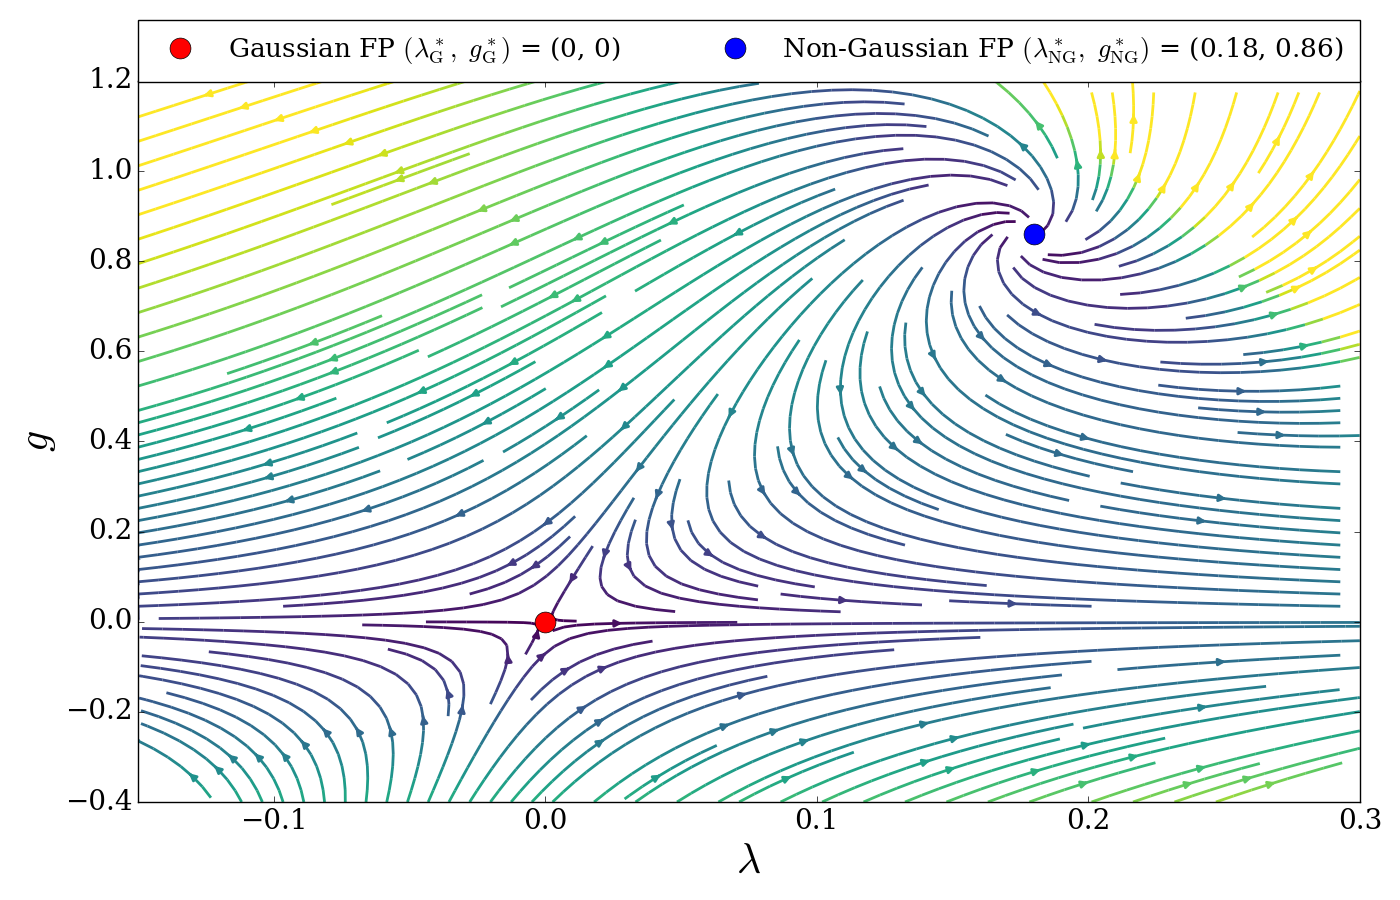
\includegraphics[width=\textwidth]{figs/Plots/EH_NoMatter}
	\caption[RG flow diagram for the Einstein-Hilbert truncation in TT approximation]{RG flow diagram  for the Einstein-Hilbert truncation in TT approximation as computed in this work. The flow points towards the infrared.}\end{figure}

%TODO: Interpretation and transition to next chapter (MATTER)